$subject$=Математическая статистика
$teacher$=Лекции Блаженова А. В.
$date$=11.03.2025

\section{Лекция 5.}

\subsection{Квантильное распределение}

Предполагаем, что распределение абсолютно непрерывное и $F(x)$ - функция распределения

\DefN{1} Число $t_\gamma$ называется квантилем распределения уровня $\gamma$, если значения
функции распределения $F(t_\gamma) = \gamma$ или $P(X < t_\gamma) = \gamma$ ($t_\gamma = F^{-1}(\gamma)$)

% https://www.geogebra.org/calculator/ezemup66

\begin{center}
    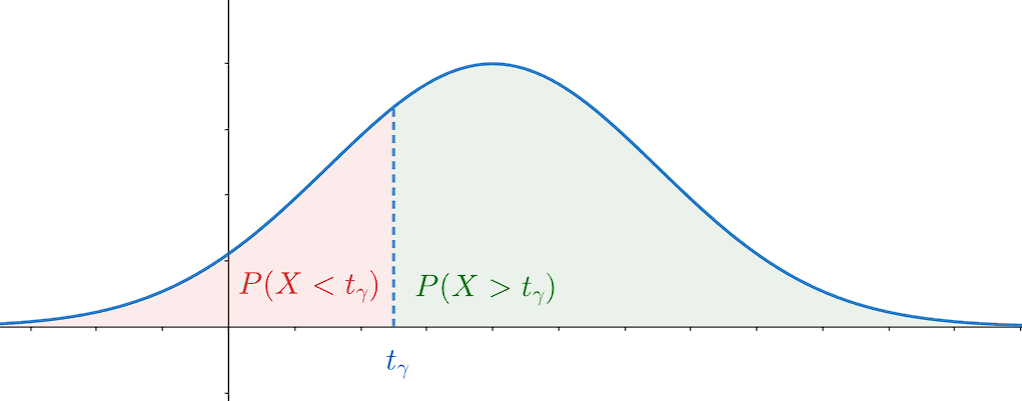
\includegraphics[width=15cm]{mathstat/images/mathstat_2025_03_11_1}
\end{center}

\Ex Медиана - квантиль уровня $\frac{1}{2}$

\DefN{2} Число $t_\alpha$ называется квантилем уровня значимости $\alpha$, если
$P(X > t_\alpha) = \alpha$ или $F(t_\alpha) = 1 - \alpha$

Ясно, что $\gamma = 1 - \alpha$

\subsection{Интервальные оценки}

Недостатки точечных оценок - неизвестно насколько они далеки от реального значения параметра и 
насколько им можно доверять. Особенно это заметно при малых выборках. Поэтому мы указываем интервал, в котором 
лежит этот параметр с заданной вероятностью (надежностью) $\gamma$. Такие оценки называются интервальными 
(доверительными)

\Def Интервал $(\theta^-_\gamma; \theta^+_\gamma)$ называется доверительным интервалом параметра $\theta$
надежности $\gamma$, если вероятность $P(\theta^-_\gamma < \theta < \theta^+_\gamma) = \gamma$

\Nota Если имеем дискретную случайную величину, то $P(\theta^-_\gamma < \theta < \theta^+_\gamma) \geq \gamma$

\Notas Так как параметр $\theta$ - константа, то бесмысленно говорить о его попадании в интервал. Правильно: 
доверительный интервал накрывает параметр $\theta$ с вероятностью $\gamma$

\NotaN{1} $\alpha = 1 - \gamma$ называется уровнем значимости доверительного интервала

\NotaN{2} Обычно пытаются строить симметричный доверительный интервал относительно несмещенной оценки $\theta^*$

\NotaN{3} Возникает вопрос, какой уровень $\gamma$ выбрать для исследования.
Стандартные уровени надежности $\gamma$: $0.9, \ 0.95, \ 0.99, \ 0.999$. Самый мейнстримный - $0.95$. 
В малых выборках используют $0.9$

Вспомним основную теорему:

\begin{MyTheorem}
    $\letsymbol (X_1, \dots, X_n)$ - выборка объема $n$ из $N(\alpha, \sigma^2)$

    $\overline{x}$ - выборочное среднее, $S^2$ - исправленная дисперсия, $D^*$ - выборочная дисперсия

    Тогда:

    \begin{enumerate}
        \item $\sqrt{n} \frac{\overline{x} - a}{\sigma} \in N(0, 1)$
        \item $\sum_{i = 1}^n \left(\frac{X_i - a}{\sigma}\right)^2 = \frac{n \tilde{\sigma^2}}{\sigma^2} \in H_n$, 
        где $n \tilde{\sigma^2} = \sum_{i = 1}^n (X_i - a)^2$
        \item $\sum_{i = 1}^n \left(\frac{X_i - \overline{x}}{\sigma}\right)^2 = \frac{(n - 1)S^2}{\sigma^2} = 
        \frac{nD^*}{\sigma^2} \in H_{n - 1}$
        \item $\sqrt{n} \frac{\overline{x} - a}{S} \in T_{n - 1}$
        \item $\overline{x}$ и $S^2$ - независимы
    \end{enumerate}
\end{MyTheorem}


\Nota Если $F(x)$ - функция симметричного относительно $x = 0$ распределения, то $P(|X| < t) = 2F(t) - 1$

% https://www.geogebra.org/calculator/msnwgfyp

\begin{center}
    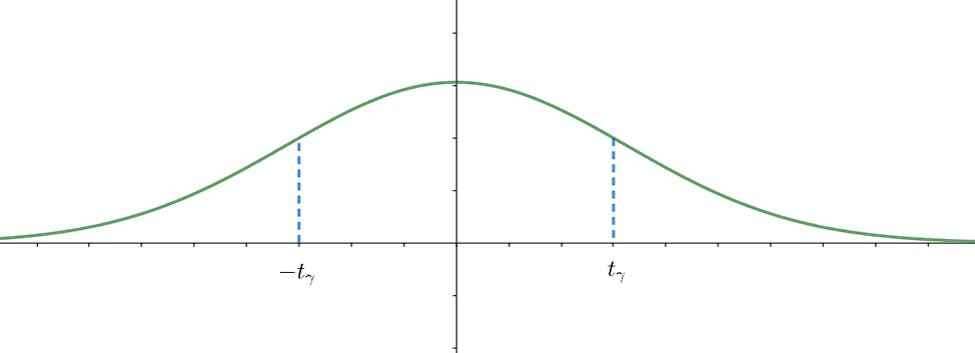
\includegraphics[width=15cm]{mathstat/images/mathstat_2025_03_11_2}
\end{center}

\subsection{Доверительные интервалы для параметров нормального распределения}

Пусть $\vec X = (X_1, \dots, X_n)$ - выборка объема $n$ из $N(a, \sigma^2)$. 
Хотим найти интервалы для параметров $a$ и $\sigma^2$

\begin{enumerate}[label*=\Roman*.]
    \item Доверительный интервал для параметра $a$ при известном значении $\sigma^2$

    По пункту 1 из теоремы $\sqrt{n} \frac{\overline{x} - a}{\sigma} \in N(0, 1)$ 

    $P\left(-t_\gamma < \sqrt{n} \frac{\overline{x} - a}{\sigma} < t_\gamma\right) = 
    P\left(\left|\sqrt{n} \frac{\overline{x} - a}{\sigma}\right| < t_\gamma\right) = 2F_0 (t_\gamma) - 1 = \gamma$

    $F_0(t_\gamma) = \frac{1 + \gamma}{2} \Longrightarrow t_\gamma$ - квантиль уровня 
    $\frac{1 + \gamma}{2}$ для $N(0, 1)$, где
    $F_0(x) = \frac{1}{\sqrt{2\pi}} \int_{-\infty}^{\infty} e^{-\frac{z^2}{2}} dz$

    Решая неравенство, получаем $-t_\gamma < \sqrt{n} \frac{\overline{x} - a}{\sigma} < t_\gamma$

    $-t_\gamma \frac{\sigma}{\sqrt{n}} < \overline{x} - a < t_\gamma \frac{\sigma}{\sqrt{n}}$

    $\overline{x} - t_\gamma \frac{\sigma}{\sqrt{n}} < a < \overline{x} + t_\gamma \frac{\sigma}{\sqrt{n}}$ - 
    симметричный интервал относительно $\overline{x}$

    Доверительный интервал надежности $\gamma$: $\left(\overline{x} - t_\gamma \frac{\sigma}{\sqrt{n}}, 
    \overline{x} + t_\gamma \frac{\sigma}{\sqrt{n}}\right)$, 
    где $t_\gamma$ - квантиль $N(0, 1)$ уровня $\frac{1 + \gamma}{2}$

    \item Доверительный интервал для параметра $a$ при неизвестном $\sigma^2$

    Из пункта 4 из теоремы $\sqrt{n} \frac{\overline{x} - a}{S} \in T_{n - 1}$

    $P\left(-t_\gamma < \sqrt{n} \frac{\overline{x} - a}{S} < t_\gamma\right) = P\left(\left|\sqrt{n} \frac{\overline{x} - a}{S}\right| < t_\gamma\right) = 2F_{T_{n - 1}}(t_\gamma) = \gamma$

    $F_{T_{n - 1}}(t_\gamma) = \frac{1 + \gamma}{2} \Longrightarrow t_\gamma$ - квантиль $T_{n - 1}$ уровня 
    $\frac{1 + \gamma}{2}$

    Аналогично с примером выше получаем интервал $\left(\overline{x} - t_\gamma \frac{S}{\sqrt{n}}, 
    \overline{x} + t_\gamma \frac{S}{\sqrt{n}}\right)$, 
    где $t_\gamma$ - квантиль $T_{n - 1}$ уровня $\frac{1 + \gamma}{2}$

    \item Доверительный интервал для параметра $\sigma^2$ при неизвестном $a$

    По пункту 3 из теоремы $\sum_{i = 1}^n \left(\frac{X_i - \overline{x}}{\sigma}\right)^2 = \frac{(n - 1)S^2}{\sigma^2} = 
    \frac{nD^*}{\sigma^2} \in H_{n - 1}$

    Пусть $\chi_1^2$ и $\chi_2^2$ - квантили $H_{n - 1}$ уровней $\frac{1 - \gamma}{2}$ и $\frac{1 + \gamma}{2}$

    Тогда $P\left(\chi_1^2 < \frac{(n - 1)S^2}{\sigma^2} < \chi_2^2\right) = F_{H_{n - 1}}(\chi_1^2) - F_{H_{n - 1}}(\chi_2^2) = \frac{1 - \gamma}{2} - \frac{1 + \gamma}{2} = \gamma$

    $\chi_1^2 < \frac{(n - 1)S^2}{\sigma^2} < \chi_2^2$

    $\frac{1}{\chi_2^2} < \frac{\sigma^2}{(n - 1)S^2} < \frac{1}{\chi_1^2}$

    $\frac{(n - 1)S^2}{\chi_2^2} < \sigma^2 < \frac{(n - 1)S^2}{\chi_1^2}$ или 
    $\frac{nD^*}{\chi_2^2} < \sigma^2 < \frac{nD^*}{\chi_1^2}$

    Получаем интервал $\left(\frac{(n - 1)S^2}{\chi_2^2}, \frac{(n - 1)S^2}{\chi_1^2}\right)$, где $\chi_1^2$ и $\chi_2^2$ - квантили $H_{n - 1}$ уровней $\frac{1 - \gamma}{2}$ и $\frac{1 + \gamma}{2}$

    \Nota Данный интервал не симметричен относительно неизвестного параметра $\sigma^2$

    \item Доверительный интервал для параметра $\sigma^2$ при известном $a$

    По пункту 2 из теоремы $\sum_{i = 1}^n \left(\frac{X_i - a}{\sigma}\right)^2 = \frac{n \tilde{\sigma^2}}{\sigma^2} \in H_{n - 1}$
    
    Пусть $\chi_1^2$ и $\chi_2^2$ - квантили $H_{n}$ уровней $\frac{1 - \gamma}{2}$ и $\frac{1 + \gamma}{2}$

    Тогда $P\left(\chi_1^2 < \frac{n \tilde{\sigma^2}}{\sigma^2} < \chi_2^2\right) = F_{H_{n}}(\chi_1^2) - F_{H_{n}}(\chi_2^2) = \frac{1 - \gamma}{2} - \frac{1 + \gamma}{2} = \gamma$

    Аналогично получаем интервал $\left(\frac{n \tilde{\sigma^2}}{\chi_2^2}, \frac{n \tilde{\sigma^2}}{\chi_1^2}\right)$, 
    где $\chi_1^2$ и $\chi_2^2$ - квантили $H_{n}$ уровней $\frac{1 - \gamma}{2}$ и $\frac{1 + \gamma}{2}$, $n \tilde{\sigma^2} = \sum_{i = 1}^n (X_i - a)^2$

    \Nota $\tilde{\sigma^2} - D^* = \frac{1}{n} \sum_{i = 1}^n (X_i - a)^2 - \frac{1}{n} \sum_{i = 1}^n (X_i - \overline{x})^2 = 
    \frac{1}{n} \sum_{i = 1}^n (X_i^2 - 2aX_i + a^2 - X_i^2 + 2 \overline{x} X_i - \overline{x}^2) = 
    \frac{1}{n} (na^2 - 2a n \overline{x} + 2 \overline{x} \cdot n \overline{x} - n \overline{x}^2) = 
    a^2 - 2a \overline{x} + \overline{x}^2 = (a - \overline{x})^2 \Longrightarrow \tilde{\sigma^2} = D^* + (a - \overline{x})^2$

    Получаем $\left(\frac{n (D^* + (a - \overline{x})^2)}{\chi_2^2}, \frac{n (D^* + (a - \overline{x})^2)}{\chi_1^2}\right)$

\end{enumerate}

\subsection{Асимптотические доверительные интервалы}

\Def Интервал $(\theta^-_\gamma, \theta^+_\gamma)$ называется асимптотическим доверительным интервалом параметра $\theta$ 
уровня $\gamma$, если $P(\theta^-_\gamma < \theta < \theta^+_\gamma) \underset{n \to \infty}{\longrightarrow} \gamma$

\Ex Доверительный интервал вероятности события $A$

Пусть $p = P(A), q = 1 - p, n$ - число испытаний или объем выборки $(X_1, \dots, X_n)$, где $X_i \in \{0, 1\}$

$p^* = \frac{n_A}{n} = \overline{x}$ - оценка $p$

Согласно Центральной предельной теореме $\sqrt{n} \frac{p^* - p}{D X_1} = \sqrt{n} \frac{p^* - p}{\sqrt{pq}} \rightrightarrows N(0, 1)$

Так как $p^* \overset{p}{\longrightarrow} p$, то $\sqrt{n} \frac{p^* - p}{\sqrt{p^* (1 - p^*)}} = 
\sqrt{n} \underset{\rightrightarrows N(0, 1)}{\underbrace{\frac{p^* - p}{\sqrt{p (1 - p)}}}} \underset{\overset{p}{\longrightarrow} 1}{\underbrace{\frac{\sqrt{p (1 - p)}}{\sqrt{p^* (1 - p^*)}}}} \rightrightarrows N(0, 1)$


$P\left(\left|\sqrt{n} \frac{p^* - p}{\sqrt{p^* (1 - p^*)}}\right| < t_\gamma\right) \underset{n \to \infty}{\longrightarrow} 2F_0(t_\gamma) - 1 = \gamma$

$F_0(t_\gamma) = \frac{1 + \gamma}{2}$, $t_\gamma$ - квантиль $N(0, 1)$ уровня $\frac{1 + \gamma}{2}$

Получаем $\left|\sqrt{n} \frac{p^* - p}{\sqrt{p^* (1 - p^*)}}\right| < t_\gamma$

$|p^* - p| < t_\gamma \frac{\sqrt{p^* (1 - p^*)}}{\sqrt{n}}$

Итак, $\left(-t_\gamma \frac{\sqrt{\overline{x} (1 - \overline{x})}}{\sqrt{n}}, t_\gamma \frac{\sqrt{\overline{x} (1 - \overline{x})}}{\sqrt{n}}\right)$, где $t_\gamma$ - квантиль $N(0, 1)$ уровня $\frac{1 + \gamma}{2}$



